
\documentclass[
	% -- opções da classe memoir --
	article,			% indica que é um artigo acadêmico
	12pt,				% tamanho da fonte
	oneside,			% para impressão apenas no verso. Oposto a twoside
	a4paper,			% tamanho do papel. 
	english,			% idioma adicional para hifenização
	brazil,				% o último idioma é o principal do documento
	]{abntex2}

\usepackage{cmap}				% Mapear caracteres especiais no PDF
\usepackage{lmodern}			% Usa a fonte Latin Modern
\usepackage[T1]{fontenc}		% Selecao de codigos de fonte.
\usepackage[utf8]{inputenc}		% Codificacao do documento (conversão automática dos acentos)
\usepackage{indentfirst}		% Indenta o primeiro parágrafo de cada seção.
\usepackage{nomencl} 			% Lista de simbolos
\usepackage{color}				% Controle das cores
\usepackage{graphicx}			% Inclusão de gráficos

\usepackage[brazilian,hyperpageref]{backref}	 % Paginas com as citações na bibl
\usepackage[alf]{abntex2cite}	% Citações padrão ABNT
\renewcommand{\backrefpagesname}{%Citado na(s) página(s):~
}
% Texto padrão antes do número das páginas
\renewcommand{\backref}{}
% Define os textos da citação
\renewcommand*{\backrefalt}[4]{
	\ifcase #1 %
%		Nenhuma citação no texto.%
	\or
		%Citado na página #2.%
	\else
	%	Citado #1 vezes nas páginas #2.%
	\fi}%
% ---

\titulo{A informação na era da Internet: possibilidades e realidades}
\autor{Elias Lima de Souza}
\local{Campinas, Brasil}
\data{Julho de 2014}

\definecolor{blue}{RGB}{41,5,195}

\makeatletter
\hypersetup{
     	%pagebackref=true,
		pdftitle={\@title}, 
		pdfauthor={\@author},
    	pdfsubject={Ei, onde sai isso aqui},
	    pdfcreator={LaTeX with abnTeX2},
		pdfkeywords={abnt}{latex}{abntex}{abntex2}{atigo científico}, 
		colorlinks=true,       		% false: boxed links; true: colored links
    	linkcolor=blue,          	% color of internal links
    	citecolor=blue,        		% color of links to bibliography
    	filecolor=magenta,      		% color of file links
		urlcolor=blue,
		bookmarksdepth=4
}
\makeatother

\makeindex

\setlrmarginsandblock{4cm}{4cm}{*}
\setulmarginsandblock{4cm}{4cm}{*}
\checkandfixthelayout

\setlength{\parindent}{1.3cm}
\setlength{\parskip}{0.2cm}

\begin{document}

\frenchspacing 
\maketitle

% resumo em português
\begin{resumoumacoluna}

Em tempos de popularização da internet, há uma percepção comum de que existem muitas informações circulando a partir de diversos meios de comunicação, permitindo que as pessoas consumam informações a partir de diferentes pontos de vista. Mas se a informação tem papel chave na estrutura capitalista atual, como ela há de ser livre de intenções? Na internet dos múltiplos emissores e receptores, recebemos conteúdo dos mesmos grupos da mídia tradicional e não exploramos a potencialidade das redes sociais para a transmissão de informações de forma consciente e livre de valor.
 
 \vspace{\onelineskip}
 
 \noindent
 \textbf{Palavras-chaves}: informação, internet, redes sociais.
\end{resumoumacoluna}

\textual

\section*{A informação como agente do capital}

Em tempos de popularização da internet, há uma percepção comum de que existem muitas informações circulando a partir de diversos meios de comunicação, permitindo que as pessoas consumam informações a partir de diferentes pontos de vista. 

A idéia de descentralização da informação é defendida por \citeauthoronline{levy1998} (\citeyear{levy1998}), ao analisar a comunicação no ciberespaço\footnote{O ciberespaço é o novo meio de comunicação que surge da interconexão mundial dos computadores. O termo especifica não apenas a infra-estrutura material da comunicação digital, mas também o universo oceânico de informações que ela abriga, assim como os seres humanos que navegam e alimentam esse universo \cite[p. 17]{levy1999}.} como um sistema ''todos para todos'', com múltiplos emissores e múltiplos receptores de conteúdo, que podem interagir com a fonte emissora, diferentemente das tradicionais imprensa escrita, televisão e rádio, onde há um agente emissor com receptores passivos.

\citeauthoronline{levy1998} (\citeyear{levy1998}, p.45) ressalta que até o surgimento do ciberespaço, o ''espaço público de comunicações era controlado através de intermediários institucionais'', e que agora, com o ciberespaço, a informação ganha um caráter coletivo, ''desintermediado''. Ele considera a internet como um espaço democrático, que todos têm acesso. A internet como possibilidade de comunicação livre.

Para \citeauthoronline{santos1996} (\citeyear{santos1996}, p. 83), a técnica atua na produção do espaço modificando-o em termos de forma, função e paisagem, fatores determinantes de novas relações entre a sociedade e o espaço e entre a sociedade e si mesma. E como ressalta \citeauthoronline{marques} (2009, p. 21), “cada lugar revela uma técnica ou um conjunto de técnicas que o caracteriza particularmente e que contribui na formação de uma identidade própria [...] desta forma, a técnica constitui um dos elementos de explicação da sociedade e de cada um dos lugares”.

Conforme \citeauthoronline{cohn2001} (\citeyear{cohn2001}, p.21-22), vivemos atualmente em uma sociedade cuja forma é sobredeterminada pela informação. E a informação é diferente da comunicação. Enquanto a comunicação tem relação com a circulação dos conteúdos, a informação tem relação com o modo como o conteúdo é incorporado (ou não) à circulação. Ou seja, a informação seleciona o que será repassado para a comunicação, ''atuando de forma decisiva na modelagem do próprio sistema capitalista'' (\citeauthor{cohn2001}, \citeyear{cohn2001}, p.22).

Hoje a informação é um elemento chave na composição da sociedade mundial e o meio técnico-científico-informacional é a “cara espacial da globalização” \cite{santos1996}, assim como a informação e os sistemas de comunicação adquirem importância fundamental na organização do espaço.

\citeauthoronline{maia} (\citeyear{maia}, p.5) ressalta ainda que a modificação acelerada do território, aliada à chegada e dispersão das técnicas de comunicação e informação, dá ao período atual uma forma diferenciada, que Milton Santos chama, em seu livro "A Natureza do Espaço", de instantaniedade dos momentos e dos lugares, universalidade e unicidade das técnicas.

\citeauthoronline{santos2001} (\citeyear{santos2001}) também trabalha com a idéia que a técnica central e dominante nos dias atuais é a técnica da informação, e que o homem deixou de ser o centro do mundo, papel hoje é exercido pelo dinheiro, em uma geopolítica proposta por economistas e defendida pela mídia (detentora da técnica da informação). Dessa forma, as grandes empresas utilizam a mídia e, conseqüentemente a técnica, para realizar um tipo de dominação sobre o território, almejando se perpetuar como agente hegemônico.

No livro A Sociedade Em Rede,  \citeauthoronline{castells1999} (\citeyear{castells1999}, p.50-51) considera a informação como um modo de desenvolvimento, moldado pela reestruturação do modo capitalista de produção, no final do século XX, que resulta no surgimento de uma nova estrutura social. Segundo o autor, a concepção teórica que fundamenta essa abordagem pressupõe que as sociedades são organizadas em processos estruturados por relações historicamente determinadas entre três elementos: a) \textbf{Produção}, baseado na ação do homem sobre a natureza para apropriar-se dela e transforma-la seu beneficio; b) \textbf{Experiência}, a ação dos humanos sobre si mesmos, determinada pela interação entre suas identidades biológicas e culturais em relação a seus ambientes sociais e naturais; c) \textbf{Poder}, relação entre humanos que, com base na produção e na experiência, impõe a vontade de alguns sobre os outros, pelo emprego potencial ou real de violência física ou simbólica.

Para o autor, a “comunicação simbólica entre os seres humanos e o relacionamento entre esses e a natureza,com base na produção (e seu complemento, o consumo), experiência e poder, cristalizam-se ao longo da história em territórios específicos, e assim geram culturas e identidades coletivas” \cite[p. 52-53]{castells1999}. Ele ainda ressalta como a difusão da tecnologia amplifica o poder de uma sociedade de forma infinita, a medida que os usuários apropriam-se da tecnologia e a redefinem: “pela primeira vez na história, a mente humana é uma força direta de produção, não apenas um elemento decisivo no sistema produtivo” \cite{castells1999}


A integração do território, motivada por interesses geopolíticos e pela necessidade de circulação de bens, pessoas e informação, deu-se através da implantação e extensão de redes geográficas, definidas por \citeauthoronline{correa} (1999) como um conjunto de localizações sobre a superfície terrestre articulado por vias e fluxos. Mais do que isso, a rede é um produto e também uma condição social, historicamente construída, dotada de intencionalidade e regulada politicamente \cite{santos1996}. \citeauthoronline{dias} (1995, p.150) frisa que a formação de redes no território é acompanhada de seletividade espacial, já que as redes não ligam todos os pontos. Elas exercem o papel de conexão de alguns pontos e de exclusão de outros, tornando mais estratégica a localização geográfica.

As redes constituem a morfologia social da sociedade atual e modificam de forma considerável a operação e os resultados dos processos produtivos e de experiência, poder e cultura. Elas são “estruturas abertas capazes de expandir de forma ilimitada, integrando novos nós desde que consigam comunicar-se dentro da rede” \cite[p. 566]{castells1999}. Essa última afirmação de Castells exemplifica o caráter excludente de uma rede, onde só é aceito o que se encaixa em seu padrão ou seus interesses. \citeauthoronline{santos1996} (1996) corrobora com essa análise, considerando as redes como agentes de inclusão e também de exclusão. \citeauthoronline{raffestin1993} (\citeyear{raffestin1993}, p.157) acredita que "toda rede é uma imagem do poder, ou mais exatamente, do poder do ou dos atores dominantes".

Para \citeauthoronline{castells1999} (1999, p. 70), as grandes áreas do mundo e consideráveis segmentos da população que estão desconectados do novo sistema tecnológico são regiões culturais e espacialmente descontínuas, enquanto grupos sociais e territórios dominantes estão constantemente conectados. Para o autor (1999, p. 476), sob a lógica do novo sistema o que importa não é a localização real dos centros de produção, mas a versatilidade de suas redes.

As sociedades são constituídas a partir das relações de poder entre seus membros, uma vez que os que detêm o poder constroem as instituições segundo seus valores e interesses. \citeauthoronline{castells2013} (2013, p.13) afirma que o “poder é exercido por meio da coerção e/ou pela construção de significado na mente das pessoas, mediante mecanismos de manipulação simbólica”.  Aqui, é importante citar \citeauthoronline{raffestin1993} (\citeyear{raffestin1993}, p. 212-213), para quem os nós não são meros pontos de conexão entre redes, mas também de poder.

Para \citeauthoronline{dantas2003} (\citeyear{dantas2003}) a partir da terceira revolução industrial, chamada de revolução da informação, a informação deixa de ser considerada um recurso e passa a ser tratada como uma mercadoria. É neste período que o marketing, a publicidade e as consultorias crescem e há uma redefinição da divisão internacional do trabalho

\begin{citacao}
Na nova etapa do desenvolvimento capitalista, as indústrias que
“puxam” a recuperação, geram empregos diretos principalmente nas atividades
de alto conteúdo intelectual: P\&D, marketing, alguns processos fabris
sofisticados. Entre os seus empregados, os de baixa escolarização são minoria,
ou não existem. Nestas indústrias, as demais atividades necessárias à fabricação
e comercialização do produto, são “terceirizadas”. Muitas dessas
atividades são transferidas para os países pobres da periferia: México,
América Central, Sudeste Asiático, em parte o Brasil. \cite[p. 21-22]{dantas2003}.
\end{citacao}

\citeauthoronline{bolano2000} (\citeyear{bolano2000}, p. 46-47) frisa que do movimento histórico de apropriação do conhecimento pelo capital surgiram duas categorias de informação. Uma está ligada diretamente ao processo de produção de mercadorias mas que não é, por si só, uma mercadoria. É uma comunicação hierarquizada, direta e objetiva. E outra categoria, que agrega como ''mais um insumo ao processo produtivo e que, controlada pelo corpo técnico e burocrático da empresa capitalista, é sempre, efetiva ou potencialmente, mercadoria-informação”.

Assim, a informação passa a ter um papel fundamental na estrutura do capitalismo, que antes era majoritariamente da indústria. E se a informação é a grande agente de produção do capital, como ela há de ser livre? A estrutura de comunicação N emissores, N receptores levantada por \citeauthoronline{levy1998} (\citeyear{levy1998}) funciona na prática? O fluxo de comunicação compreende todas as informações ou uma informação dotada de intencionalidades nem sempre claras ao receptor?

\section*{A Internet com intencionalidade}

Ao analisar as teorias de Milton \citeauthoronline{santos2001} (\citeyear{santos2001}), \citeauthoronline{pasti2013} (\citeyear{pasti2013}, p. 3) ressalta que ''mesmo com o aparente “excesso” quantitativo de notícias circulando no território, a informação sobre o que acontece não vem da interação entre as pessoas, mas do que é veiculado pela mídia, com uma interpretação interessada dos acontecimentos''.

Mas se a internet, ao menos em teoria, permite a comunicação livre, de indivíduo para indivíduo, porque ela não acontece? O Observatório da Imprensa realizou uma pesquisa\footnote{Pesquisa Brasileira de Mídia 2014. Disponível em: http://observatoriodaimprensa.com.br/download/PesquisaBrasileiradeMidia2014.pdf. Acesso em 30. jun. 2014} sobre o uso da mídia pelo brasileiro, que apresenta, entre outros dados, os endereços de internet mais acessados pelos brasileiros como fonte de informações.

Dentre os cinco mais acessados, temos: 

\begin{enumerate}
\item A rede social americana Facebook;
\item O portal de entretenimento e notícias Globo.com;
\item O portal de notícias G1 (interno ao Globo.com);
\item O portal Universo On Line, que serve de acesso para à Folha de São Paulo;
\item A versão brasileira do portal norte-americano Yahoo.
\end{enumerate}

Dentre os outros sites mais acessados, também se destacam páginas como Youtube, ligado ao Google e páginas que pertencem às Organizações Globo, como Globo News Online, Ana Maria e Globo Online. O Twitter e os portais Terra, R7 (do grupo Record) e Abril.com também figuram na lista dos vinte mais acessados pelos brasileiros como fonte de informações.

Este resultado mostra que na internet, o brasileiro utiliza redes sociais e portais de grupos que já dominam outros meios de informação para se informar. Tomando por exemplo as Organizações Globo, que aparece com grande destaque na lista citada. Obviamente, conteúdo do portal Globo.com segue as mesmas diretrizes do canal de TV Globo, da rádio Globo e do jornal impresso O Globo. É claro que o grupo faz um trabalho coordenado, onde um veículo de comunicação promove o outro e o portal na internet atua como agregador de todos.

E o mesmo acontece, em diferentes proporções, com os outros sites. Estes são os mais acessados porque são os mais promovidos, os que possuem ações de marketing e publicidade. 

Ao final, todos os sites citados apresentam informações para a massa, o que \citeauthoronline{bolano2000} (\citeyear{bolano2000}, p. 55) considera como unidirecional, uma informação que “se transforma em instrumento de dominação no sentido técnico do termo”. É a internet, teoricamente multidirecional, sendo trabalhada de forma unidirecional.

Claro que a internet permite uma interação maior entre os emissores e receptores da comunicação, mas o que vemos nas seções de comentários das notícias destes portais não é um debate sadio. \citeauthoronline{ribeiro1991} (\citeyear{ribeiro1991}, p. 47), ao analisar a expansão da televisão brasileira nos anos 1980, fala sobre o poder exercido pelos processos de comunicação sobre a sociedade. Se na época a possibilidade de estar em cena para milhões de pessoas era um apelo quase irresistível (vide a mobilização de pais para que seus filhos aparecessem em programas infantis da época), hoje podemos traçar um paralelo entre o apelo de outrora e a possibilidade atual de postar comentários e publicações na internet.

A partir desta necessidade de comentar e compartilhar conteúdo na internet, verificamos páginas nas redes sociais com muitos seguidores e com postagens de rápida leitura, superficiais e muitas vezes com conteúdo falso. Ora, a pesquisa citada anteriormente coloca o Facebook como o site mais acessado pelos brasileiros que utilizam a web para se informar e temos nessa rede páginas com muitos seguidores recebendo e compartilhando conteúdo potencialmente falso, que tipo de informação os brasileiros que utilizam a internet estão consumindo?

Podemos tomar como exemplo a página TV Revolta\footnote{https://www.facebook.com/tvrevolta}, com mais de 3 milhões de seguidores. Ali são veiculadas entre frases de auto-ajuda e imagens dóceis, montagens - que em geral contém fotos de personalidades da política brasileira - com frases curtas contra programas sociais, a democratização da mídia e os direitos humanos. Esse tipo de publicação gera uma falsa sensação de informação ao receptor menos atento e, por ser de rápida leitura, atinge um público maior. Em uma projeção simples, se 10\% do público que segue esta página compartilhar uma postagem com fatos levianos, temos a rede de contatos de 300 mil pessoas com visibilidade à esse conteúdo.

A TV Revolta é um agente de poder da estrutura midiática brasileira. Mas ela atua mais como um agente de desinformação devido ao conteúdo muitas vezes falso e ao teor ofensivo de suas postagens, do que de informação. É possível mensurar a importância dessa divulgação de informações levianas para a sociedade? E para a estrutura política brasileira?

Logo após as eleições presidenciais de 2010, foi vinculado na web um mapa do Brasil (Figura 1) com os estados em azul ou vermelho, de acordo com o partido (PT ou PSDB) que teve mais votos na região. A imagem mostra que os estados do Norte e Nordeste do país foram os responsáveis pela eleição de Dilma Roussef (PT), enquanto os estados do sul e centro-oeste os opositores.

A partir desse tipo de publicação tivemos várias manifestações preconceituosas nas redes sociais. Uma delas\footnote{http://www1.folha.uol.com.br/fsp/poder/43359-estudante-de-direito-e-condenada-por-ofensa-a-nordestinos-no-twitter.shtml. Acesso em 01.jul.2014}, feita por uma estudante de direito, tomou grandes proporções e a estudante foi condenada por racismo na justiça. 

\begin{figure}[ht!]
\centering
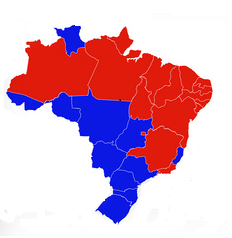
\includegraphics[width=70mm,height=70mm]{mapa_1.png}
\caption{Mapa do Brasil Eleições 2010 - I. Adaptado de http://tinyurl.com/ohdgu3b. Acesso em 01.jul.2014}
\label{overflow}
\end{figure}

O problema da Figura 1 é que ela representa os votos por estado de maneira absoluta. Como se todos em São Paulo tivessem votado no PSDB e todos em Pernambuco votado no PT. Ele mais desinforma do que informa e, para corrigir isso, o site Conversa Afiada\footnote{http://www.conversaafiada.com.br} publicou um mapa (Figura 2) que exibe os votos por partido de forma proporcional em cada estado.

Agora conseguimos ver um Brasil roxo ao invés de azul e vermelho. Ou seja, não existe o regionalismo partidário no contexto das eleições de 2010, como o mapa anterior mostra.

\begin{figure}[ht!]
\centering
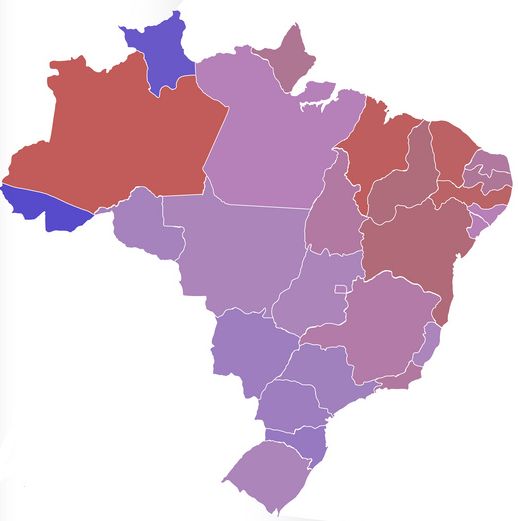
\includegraphics[width=60mm,height=60mm]{mapa_2.png}
\caption{Mapa do Brasil Eleições 2010 - II. Adaptado de http://tinyurl.com/ohdgu3b. Acesso em 01.jul.2014}
\label{overflow}
\end{figure}

É claro que com a internet existe mais espaço para mídias alternativas do que em outros meios de comunicação. Todavia, esse espaço ainda é mais potencial do que real já que ainda não sabemos aproveitar a internet da forma como ela pode ser aproveitada. Talvez a sociedade ainda não esteja pronta para emitir e consumir informações, questionando a origem e a veracidade das mesmas. 

Nesse sentido, \citeauthoronline{boaventura2005} (\citeyear{boaventura2005}) analisa o uso das novas tecnologias de comunicação e de informação como 

\begin{citacao}
uma enorme oportunidade e um enorme risco. Uma não é possível sem o outro, mas é possível maximizar as oportunidades e minimizar os riscos. Para isso, é necessário criar e aplicar generalizadamente níveis de competência técnica e política nos cidadãos muito acima daqueles que a democracia liberal até agora foi capaz de gerar \cite[p.90]{boaventura2005}
\end{citacao}

O mesmo autor (\citeyear{boaventura2005}, p. 91) ainda justifica o uso das tecnologias pois elas "criam oportunidades insuspeitadas para desenvolver competência cidadã, competência para deliberar e tomar decisões políticas e não apenas para escolher os decisores políticos".

Hoje, para obter uma informação de fora dos principais emissores, é necessário procurar um pouco mais. Ainda de forma tímida, mas em constante crescimento, temos grupos como a Mídia Ninja\footnote{http://www.midianinja.org/} e o Coletivo Intervozes\footnote{http://intervozes.org.br/}, entre outros, exercendo o papel de mídia alternativa aos grandes grupos através principalmente das redes sociais. 

São projetos mais ligados às ideias apresentadas por \citeauthoronline{dantas2003} (\citeyear{dantas2003}, p. 40), onde a informação deve circular na internet como um presente (compartilhada) e não como valor. Porém, para se ter uma idéia da dimensão e alcance desses grupos, em Junho de 2014, o Facebook da Mídia Ninja possuia cerca de 290 mil seguidores e o do Intervozes, 9 mil. Já a TV Revolta, como foi exposto anteriormente, possui mais de 3 milhões adeptos.

\bookmarksetup{startatroot}
\bibliography{bibliografia-artigo}
\end{document}